%%%%%%%%%%%%%%%%%%%%%%%%%%%%%%%%%%%%%%%%%
% University/School Laboratory Report
% LaTeX Template
% Version 3.1 (25/3/14)
%
% This template has been downloaded from:
% http://www.LaTeXTemplates.com
%
% Original author:
% Linux and Unix Users Group at Virginia Tech Wiki 
% (https://vtluug.org/wiki/Example_LaTeX_chem_lab_report)
%
% License:
% CC BY-NC-SA 3.0 (http://creativecommons.org/licenses/by-nc-sa/3.0/)
%
%%%%%%%%%%%%%%%%%%%%%%%%%%%%%%%%%%%%%%%%%

%----------------------------------------------------------------------------------------
%	PACKAGES AND DOCUMENT CONFIGURATIONS
%----------------------------------------------------------------------------------------

\documentclass{article}

\usepackage[version=3]{mhchem} % Package for chemical equation typesetting
\usepackage{siunitx} % Provides the \SI{}{} and \si{} command for typesetting SI units
\usepackage{graphicx} % Required for the inclusion of images
\usepackage{natbib} % Required to change bibliography style to APA
\usepackage{amsmath} % Required for some math elements 
\usepackage[margin=1in]{geometry}
\usepackage{hyperref}
\usepackage[british]{babel}
\selectlanguage{british}

\setlength\parindent{0pt} % Removes all indentation from paragraphs

\renewcommand{\labelenumi}{\alph{enumi}.} % Make numbering in the enumerate environment by letter rather than number (e.g. section 6)

%\usepackage{times} % Uncomment to use the Times New Roman font

%----------------------------------------------------------------------------------------
%	DOCUMENT INFORMATION
%----------------------------------------------------------------------------------------

\title{Computer Vision - Lab 2 \\ Camera Calibration} % Title

\author{Davide Dravindran Pistilli} % Author name

\date{\today} % Date for the report

\begin{document}

\maketitle % Insert the title, author and date

\section{Introduction}
This lab experience was performed to calibrate a camera from a given set of checkerboard images and to remove distortion from a test image using the previously computed calibration data.

\section{Procedure}
The first step, after loading the calibration dataset, is to find all corners in each image. This is done in parallel on 4 separate threads, since each image is independent from the others. Furthermore, after locating all corners, their coordinates are refined through the use of the function \texttt{cv::cornerSubPix}.
When all images are correctly processed, the actual calibration data are computed through the function \texttt{cv::calibrateCamera}.
The program was tested with two different input configurations: \textbf{Test A} only contained the first 12 images from the dataset, while \textbf{Test B} contained all 57 of them.
This was done to get an idea about the impact of a much larger dataset on camera calibration.

\section{Results}
\textbf{Test A} provided the parameters displayed in \textit{Figure \ref{img_data_12}} and was completed in around $1.5s$.

\begin{figure}[h]
\begin{center}
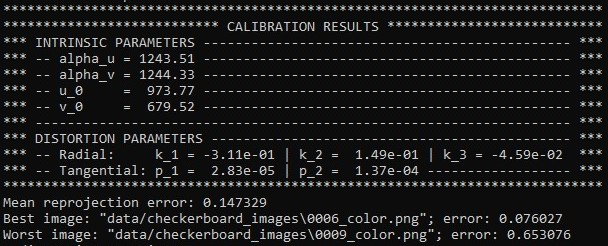
\includegraphics[width=1\textwidth]{images/data_12}
\caption{\footnotesize{calibration data with 12 input images.}}
\label{img_data_12}
\end{center}
\end{figure}

\textbf{Test B} provided the parameters displayed in \textit{Figure \ref{img_data_57}} and was completed in around $22s$.

\begin{figure}[h]
\begin{center}
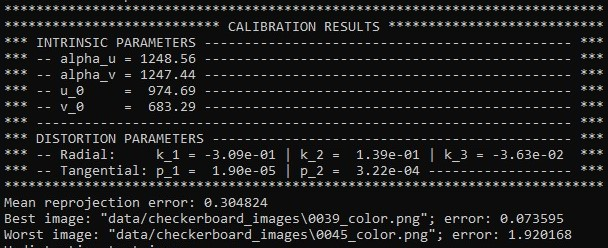
\includegraphics[width=1\textwidth]{images/data_57}
\caption{\footnotesize{calibration data with 57 input images.}}
\label{img_data_57}
\end{center}
\end{figure}

The results from distortion removal can be seen in \textit{Figures \ref{img_result_12}} and\textit{ \ref{img_result_57}}.

\begin{figure}[h]
\begin{center}
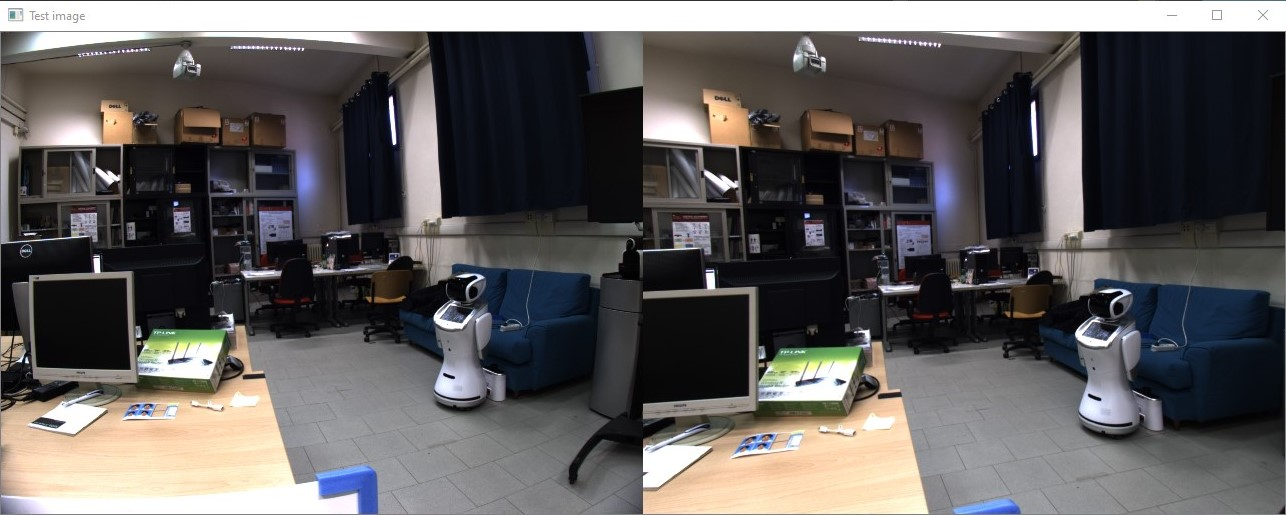
\includegraphics[width=1\textwidth]{images/result_12}
\caption{\footnotesize{distortion removal after calibration with 12 images.}}
\label{img_result_12}
\end{center}
\end{figure}

\begin{figure}[h]
\begin{center}
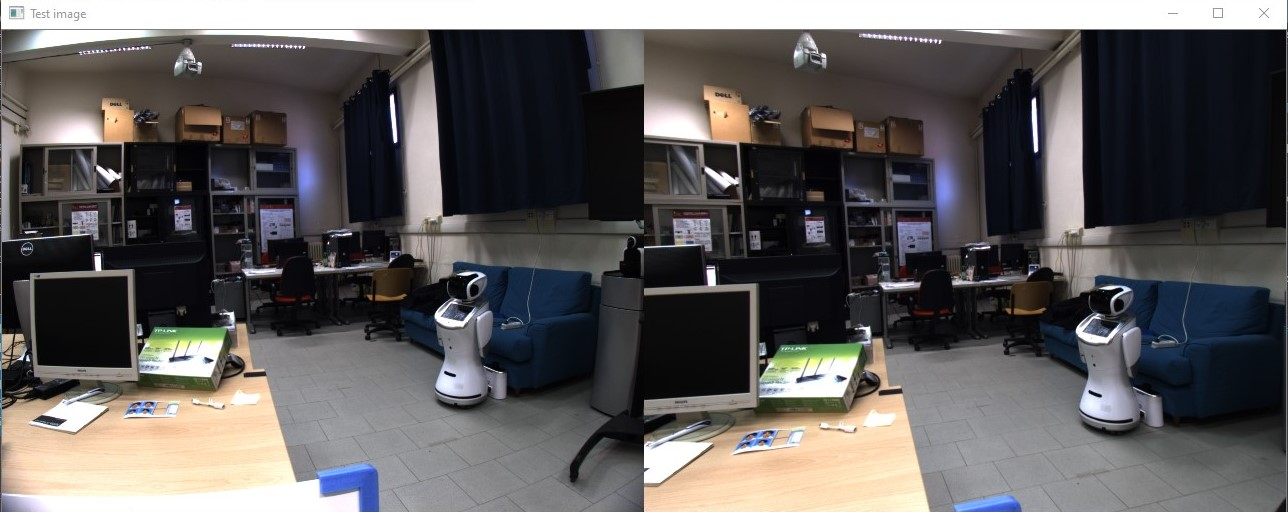
\includegraphics[width=1\textwidth]{images/result_57}
\caption{\footnotesize{distortion removal after calibration with 57 images.}}
\label{img_result_57}
\end{center}
\end{figure}

The output images are almost identical, but if we look at the data, we notice that calibrating with too many images actually has a negative impact on the reprojection error. Furthermore, \textbf{Test B} was almost $15$ times slower than \textbf{Test A}.
This means that the optimal amount of images for camera calibration has to be chosen carefully in order to avoid overfitting.

\end{document}